%!TEX root=../documentation-bachlorthesis-speicherarchitektur-lstucker.tex
\cleardoublepage
\chapter{Speicherarchitekturen}

Die heutigen bekannten Speicherarchitekturen können in Block- (Block-Based), Datei- (File-Based) und Objekt-Basierende adressierende Systeme unterteilt werden.

\section{Block-Basierend}
Die Block-Basierende Speicherarchitektur ist wohl die traditionellste und weit verbreitetste Form zum Speichern und Zuzugreifen von Daten. Die meisten Computersysteme, sei es Server, Desktop-PCs, Tablet-PC, Smartphones, Spielkonsole, speichern Ihre Daten in einen Blockbasierenden Speicher ab. Als Speicher werden in diesen Geräte meist magnetischen Festplatten, Solid State Disk oder Flash-Speicher eingesetzt.

Bei Block-Speicher werden Daten in Blöcke gelesen und gespeichert (adressiert), ein Block bildet sich aus einer Sequenz von Bits bzw. Byte. Die Grösse eines Blocks wird als Blocklänge bezeichnet, und ist bei allen Blöcken einer Einheit gleich gross. 

Experten wie Mike Mesnier, Greg Ganger und Erik Riedel, sehen jedoch bei zunehmender Speichergrösse und Komplexität von Systemen fundamentale Limitierungen von Block Schnittstellen.

\begin{quotation}
\em Since the first disk drive in 1956, disks have grown by over six orders of magnitude in density and over four orders in performance, yet the storage interface (i.e., blocks) has remained largely unchanged. Although the stability of the block-based interfaces of SCSI and ATA/IDE has benefited systems, it is now becoming a lim- iting factor for many storage architectures. As storage infrastructures increase in both size and complexity, the functions system designers want to perform are fundamentally limited by the block interface. \end{quotation}\cite{Mesnier2003}

Vergleicht man die erste Festplatte, welche von IBM produziert wurde, mit einer Seagate von 2011, hat sich die Speicherdichte von 2000 bit per Quadratzoll auf 625 Gigabyte und in der Geschwindigkeit von 8 Kilobyte auf 600 Megabyte verbessert\cite{Seagate2011}\cite{Seagate2011a}

Für den Zugriff auf Blockbasierende Speichersysteme werden meist Schnittstellen Protokolle wie Small Computer System Interface (SCSI) oder Advanced Technology Attachment (ATA) verwendet. Diese Protokolle wurden jedoch in einer Zeit entwickelt, wo man davon ausging, dass ein Block Speicher jeweils nur von einem Computersystem verwendet wurde und nicht mit mehreren Computersystemen geteilt wird. Dies Annahme stimmt in Consumer Elektronik Bereich meist noch heute, in Bereichen wo jedoch grosse Speicherkapazitäten oder eine grössere Verfügbarkeit gefordert ist, wie Sie im Geschäftsbereich vorkommen, stimmen diese Annahmen nicht mehr.

Blockbasierende Speicher, welche nicht aus Internen Speicher eines Server gebildet werden, unterscheidet man in Direct Attached Storage (DAS) und Storage Area Network (SAN). 

\subsection{Direct Attached Storage}
Bei DAS handelt es sich, wie es aus der englischen Bezeichnung zu entnehmen ist, um Speicher, welche direkt an ein Computersystem angeschlossen wird. Bei DAS Enclosure handelt sich um ein Gehäuse mit mehren verbauten Festplatten, welche üblich über einen Host-Bus-Adapter an ein Computersytem angeschlossen wird. Als Schnittstellen Protokoll werden ATA, STA, eSATA, SCSI, SAS und Fibre Channel eingesetzt. DAS können mit mehreren Computersystemen geteilt werden, sofern genügen Schnittstellen zur Verfügung stehen.


\subsection{Storage Area Network}
Die Storage Networking Industry Association (SNIA) definiert ein Storage Area Network (SAN) als ein Netzwerk, welch primärer Bestimmungszweck ist Daten zwischen Computersysteme und Speicherelemente und unter Storage Elemente zu transferieren. Ein SAN besteht aus einer Kommunikations-Infrastrukture, welches eine physische Verbindung und eine Management-Schicht beinhaltet, welches die Verbindungen, die Speichereinheiten und das Computersystem organisiert, sodass der Datentransfer sicher und robust erfolgen kann. Der Begriff SAN wird normalerweise (aber nicht notwendigerweise) mit dem Block I/O Service in Verbindung gebracht und weniger mit dem Datei-Zugriff-Service.\cite{SNIA2011}

Je nach SAN Implementierung kommen folgende Geräte bzw. Komponenten vor:
\begin{itemize}
\item Server
\item Host Bus Adapter
\item Gigabit Interface Converter
\item SAN-Switch
\item Speichersystem
\item Tape Library
\item Logical Unit
\end{itemize}

\paragraph*{Server} 
Der Server greift über das SAN auf Ressourcen von Speichersystem oder Tape Library. In einzelnen Fällen kann der Server selbst über SAN anderen Server Speicher zur Verfügung stellen.

\paragraph*{Host Bus Adapter}
Host Bus Adapter (HBA) für das SAN sind intelligente Hardwareschnittstellen, welche für die Verbindung von Server in einem SAN verwendet werden. Sofern die Server nicht bereits mit einen Host Bus Adapter ausgerüstet sind, können die meisten durch Host Bus Adapter in form von Steckkarten erweitert werden. Der Host Bus Adapter selber hat pro Port ein Einschub in welche ein Gigabit Interface Converter eingebaut wird. \cite{Christopher2009}

\paragraph*{Gigabit Interface Converter}
Der Gigabit Interface Converter sind modulare Schnittstellen, welche Elektrische Signale in optische Signale umwandeln.\cite{SNIA2011}

\paragraph*{SAN-Switch}
Der SAN Switch ist ein Switch, welche dezidiert für das SAN Umgebung verwendet wird.

\paragraph*{Speichersystem}
Das Speichersystem stellt im SAN den geteilten Speicher zur Verfügung. Gemäss den IT Marktforschung und Analyse Unternehmen Gartner gehören EMC, IBM, NetApp, Dell, HP, Hitachi zu den Marktführer\cite{RogerW.CoxPushanRinnenStanleyZaffos2011}.

\paragraph*{Tape Library}
Tape Library sind Bandbibliothek in welche ein oder mehre Bandlaufwerke und mehrere Magnetbänder befinden und der automatische Bandwechsel mittels eines Roboter realisiert wird. Die Tape Library werden für die Sicherung von Daten auf Band eingesetzt.

\paragraph*{Logical Unit}
Ein Logical Unit ist ein Gerät, welche über SCSI Protokoll andressiert mittel Logical Unit Number (LUN) wird, weshalb oft auch wenn technisch nicht korrekt das Gerät als LUN bezeichnet wird. Im Speichersystem werden mehre Festplatten mittels RAID zu einer Einheit zusammengefasst, sofern keine weitere Virtualisierung von dem Speicherhersteller zum Einsatz kommt, wird die zusammengefasste Einheit wiederum in Speichereinheiten aufgeteilt und diese als LUN dem Server zugeteilt.\cite{SNIA2011}

\subsubsection{Fibre Channel}
SCSI ist zwar sehr populär, ist jedoch mit 80 Mbps Geschwindigkeit, maximal 25 Meter Bus länge, und mit maximal 32 Geräte pro Bus, ein limitierender Faktor für viele Anwendungen. Unteranderem wegen erwähnten Limitierungen von SCSI hat, das American national Standards Institute (ANSI) die Fibre Channel Technik entwickelt. Fibre Channel ist ein mehrschichtiges Netzwerk, welche die Charakteristische und Funktionen für die Übertragung von Daten über ein Netzwerk definiert. Der Standard beinhaltet von der physikalischen Schnittstelle, Daten Codierung, Übertragungssteuerung (Link Control), Fluss Kontrolle, bis hinzu den Protokoll Schnittstellen. In Vergleich zu anderen Netzwerken, beinhaltet die Fibre Channel Architektur einen signifikanten Anteil von Hardware Prozesse um eine hohe Performance zu erreichen.\cite{Gupta2002}\cite{Christopher2009}

Beim Design von Fibre Channel hat man darauf geachtet die Besten charakteristischen Eigenschaften von I/O Bus Kommunikation (Channel) zwischen zwei Geräte und der Netzwerk Kommunikation zwischen Mehren Geräte zu kombinieren. Die Channel Kommunikation ist im Vergleich zur Netzwerk-Kommunikation, Hardware-Intensive, schnell und produziert wenig Overhead. Netzwerk Kommunikation ist hingegen, abhängig von der Software Implementierung genannt Protokoll, unterstützt aber die Kommunikation von einer grossen Anzahl Geräten.

Anders wie es der Namen von Fibre Channel vermuten lässt, ist Fibre Channel nicht auf Fiberoptik-Kabel als Kommunikations-Medium beschränkt, sondern lässt sich auch auf Kupferkabel betreiben. Aufgrund von physikalischen Eigenschaften ist hier Fiberoptik-Kabel in Geschwindigkeit kombiniert mit Distanz dem Kupferkabel überlegen. So liegt die maximale Distanz bei Kupferkabel bei 30 Metern bei einer Geschwindigkeit von 1 Gbps, bei höheren Geschwindigkeiten wird die maximale Distanz noch weiter reduziert. Bei Fiberoptic-Kabel wird die maximale Distanz von Fiberoptic-Kabel-Typ, Lichtwellenlänge Rundreise Latenz und eingesetzter Hardware bestimmt. Bei einen 


diese bei 10 Kilometer. Mit spezieller Hardware können auch Distanzen von bis zu 600 Kilometer \footnote{\url{http://www.enterprisestorageforum.com/industrynews/article.php/2171801/Synchronous-SAN-Sets-Fibre-Channel-Distance-Record.htm}} erreicht werden, wobei neben der Geschwindigkeit auch die grösser werdende Latenz ein limitierender Faktor ist. Für eine Distanz von 600 Kilometer braucht das Licht im Vakuum $ \approx 200.138\mu s$, in einer Fiberoptic-Kabel wird dieser Wert noch höher sein.????
Eine Fibre Channel SAN besteht aus diesen Grund in der Regeln aus Fiberoptic  Verbindungen.

Es gibt drei Fibre Channel Topolgien:
\begin{itemize}
\item Point-to-Point
\item Arbitrated-Loop
\item Switched-Fabric
\end{itemize}

\paragraph*{Point-to-Point-Topologie}
Die Point-to-Point-Topologie ist die direkte Verbindung von zwei Fibre Channel Geräte, meistens handelt es sich bei der Verbindung von einem Server und einen Speichersystem, wie Sie im Direct Attached Storage (DAS) Umfeld vorkommt. \cite{Christopher2009}

\paragraph*{Arbitrated-Loop-Topologie}
Bei der Arbitrated-Loop-Topologie können bis zu 126 Knoten (NL\_Ports) an einen geteilten Bus Ring zusammengeschlossen werden. In diesen Ring kann eine Verbindung zwischen zwei Ports aktive sein, alle anderen Ports fungieren währende diese Verbindung aktive ist als Repeater und leiten das Signal weiter. Die Arbitrated-Loop-Topologie ist deshalb von der Architektur ähnlich wie dem Token Ring.\cite{Gupta2002}\cite{Christopher2009}

\paragraph*{Switched-Fabric-Topologie}
Die Klassischen SAN Topologie ist die Switched-Fabric-Topologie. Eine Switched-Fabric-Topologie besteht aus einer oder mehreren Switches die zu einer Fibre Channel Fabric zusammengeschlossen werden. Die einzelnen FC-Geräte, wie Server bzw. Storagesystem, werden über eine oder mehre Ports an eine Switched Fabric angeschlossen. In eine Fabric können bis zu $2^{24}$ Ports angeschlossen werden.\cite{Gupta2002}\cite{Christopher2009}

Mit der Switched-Fabic-Topologie lassen sich verschiedene Fabric Topologien bilden.
Die einfachste Topologie, welche das Design Ziel die Eliminierung von Single "'Point of Failure"' erfüllt, ist die Dual Switch Topologie, wie in der \refabb{abb:DualSwitchTopologie} dargestellt dient jeder Switch als eigenständige Fabric. Die FC-Geräte wie Server und Storagesystem werden jeweils pro Fabric bzw. Switch mit mindestens einen FC-Port angeschlossen. Durch den Einsatz von Path Management Software auf dem Server, kann eine vom Speichersystem zugeteiltes Logical Unit über mehre Path angesprochen werden. Diese Implementierung bietet gleich mehre Vorteile. Wenn ein Path oder eine ganze Fabric ausfällt übernimmt der andere Path automatisch für den ausgefallen Path. Bei Wartungsarbeiten an Komponenten einer Fabric kann der Service ohne Downtime weiter betrieben werden. Moderne Path Management Software und Speichersystem unterstützen zudem die Lastverteilung (Loadbalance) des I/O Last über alle Pathe.\cite{Christopher2009}

\begin{center}
\includegraphics[width=\linewidth, keepaspectratio = true]{media/}
\mycaption{figure}{\label{abb:DualSwitchTopologie}Fibre Channel SAN mit Dual Switch Topologie}
\end{center}

Die Meshed Fabric Topologie erhöht die Ausfallsicherheit zusätzlich innerhalb den einzelne Fabric. Für die Meshed Fabric sind pro Fabric mindestens vier Fibre Channel SAN Switches erforderlich. Jeder Switch wird wie in \refabb{abb} ersichtlich ist mit mindestens einen Path, den sogenannten Inter Switch Link (ISL), zu allen anderen Switches in der Fabric Verbunden. Die Meshed Fabric kann den Ausfall von Mehren Kabel und Switch verkraften ohne das die ganze Fabric ausfällt.\cite{Christopher2009}

\begin{center}
\includegraphics[width=\linewidth, keepaspectratio = true]{media/}
\mycaption{figure}{\label{abb:MashedFabricTopologie}Fibre Channel SAN mit Mashed Fabric Topologie}
\end{center}

\subsubsection{iSCSI}
Das SCSI-Protokoll ist ein populäres Protokoll für die Kommunikation mit I/O Geräten, spezielle für Speicher Geräte. SCSI weist die Client-Server Architektur auf, wobei der Clients bei SCSI Interface als "initiators" bezeichnet wird und die logische Einheit vom Server als "target".

SCSI Protokoll wurde schon über Protokolle transportiert, jedoch waren all die Transport Protokolle limitiert in der Distanz. IBM startete 1996 mit der Forschung für die Übertragung von SCSI über das Ethernet, dabei untersuchte IBM ob sich der Transport mittels IP oder TCP/IP besser eignen würde. Messungen zeigte da zumal, dass in einem lokalen Netzwerk, der Transport mittels IP besser eignet, anstelle von TCP/IP, mit der Extrapolation in die Zukunft, und den Transport über die lokale Netzwerkgrenze hinweg war aber der Weg mittels TCP/IP die bessere Wahl. 1999 hatten sich IBM und Cisco geeinigt "SCSI over TCP/IP" gemeinsam in eine Internet Engineering Task Force Standart weiter zu entwickeln. \cite{JohnL.202} Die fertige Spezifikation von SCSI over TCP/IP ist im RFC 3720 mit dem Namen iSCSI in April 2004 fertiggestellt worden.\cite{J.Satran2004}

\paragraph*{Kosten}
Für den Betrieb eines Fibre Channel SAN sind spezielle Hardware und Fibre Channel Kenntnis notwenig. Aufgrund, dass bei iSCSI die selbe Technik wie im Computernetzwerk verwendet wird, benötigt es für den Betrieb keine zusätzliche Ausbildung, Netzwerk Infrastruktur und Management Software Lösungen, was die Gesamtbetriebskosten (TCO) senkt.

Grundsätzlich kann jeder Computer, welcher mit einem Netzwerkanschluss ausgerüstet ist und einen iSCSI Software Treiber hat, iSCSI nutzen. Computer welche Genügen Prozessor Leistung haben können die zusätzliche Last für die Verarbeitung von iSCSI mit konventionellen Netzwerkkarten lösen. Bei Computersystem, welche die Verarbeitungsgeschwindigkeit kritisch ist, wie bei Server kann diese zusätzliche Last negativ sein. Vergleichbar wie für Fibre Channel gibt es für iSCSI spezielle Netzwerkkarten bzw. Host Bus Adapter, welche mittels TCP/IP Offload Engine (TOE) und volle iSCSI Offload Engine im eignen Chip die TCP/IP bzw. iSCSI Pakete verarbeiten. Solche Netzwerkkarten entlasten durch die Verarbeitung der TCP/IP und iSCSI Pakete im eignen Chip die Central Processing Unit (CPU) des Servers und weisen bessere Werte in der Latenz auf.

\paragraph*{Netzwerk}
In einem Ethernet Netzwerk verwaltet sich jeder Switch mehr oder weniger autonome und führt eine eigene Weiterleitungstabelle, mit welcher der Switch entscheidet, über welchen Port eine Ethernet Packe ausgeliefert werden muss. Dazu enthält die Weiterleitungstabelle pro MAC Adresse den dazugehörigen Port. Trifft eine Ethernet Paket mit noch unbekannter MAC Adresse ein, leitet der Switch das Paket über alle Ports weiter. Durch die Rückantwort des Zielsystems lernt der Switch, über welchen Port, das System erreichbar ist. Werden in einen Switch Netzwerk benachbarte Switches untereinander über mehre Pfade Verbunden, kann es bei in einen solchem Szenario eintreffen, dass das Paket wieder am ursprünglichen Switch ankommt, wenn der benachbarte Switch die MAC-Adresse ebenfalls nicht kennt. Es entsteht dadurch eine Verdoppelung, der Ethernet Paket im Netzwerk bzw. es kommt zu einer Schleifenbildung, was wiederum zu Netzwerkstörungen führt. Mittels Spanning Tree Protokoll (STP) sollen solche Schleifen vermieden werden. Das Spannung Tree Protokoll erstellt eine Baum Topologie mit jeweils einer aktiven Path zwischen zwei Switches. Diese Topologie hat mehre Nachteile: 

\begin{itemize}
\item Beim Topologie-Wechsel wird im Netzwerk der Spanning Tree neu ausgehandelt, während dieser Neuaushandlung kommt es zu einem mindestens 15-Sekunden-Unterbruch. In dieser Zeit werden keine Ethernet Paket weiter geleitet. Eine Topologie Wechsel kann, zum Beispiel durch einen Pfad Ausfall zwischen zwei Switches hervorgerufen werden.

\item In einer Baum-Hierarchie, müssen die Pakete innerhalb des Baumes weitergeleitet werden und können nicht über einen theoretisch direkteren Pfad weitergeleitet werden. Befindet sich das Ziel auf der anderen Baum Seite, muss das Paket die ganze Hierarchie hinauf weitergeleitet werden und auf der anderen Seite hinunter bis zum Ziel System. Könnten die Switches über mehre Pfade miteinander Kommunizieren, könnte ein direkter Weg gewählt werden und in der Kommunikation währen weniger Switches belastet.
\end{itemize}

Hersteller wie Brocade haben diese Problematik für den Betrieb von iSCSI SAN erkannt und haben Lösungen entwickelt welche das Prinzip von Fibre Channel Fabrics für Ethernet Netzwerke umsetzen. Bislang ist darauf jedoch noch keinen allgemeinen Standard entstanden, weshalb es bei solchen Lösungen um porträtiere Lösungen handelt.

\paragraph*{Sicherheit}
Wie beim Fibre Channel SAN sollte im Geschäftsumfeld iSCSI über ein dediziertes Netzwerk laufen. Die Abgrenzung erhöht die Sicherheit, das Storage Netzwerk ist somit klar abgeschottet von restlichen Netzwerken. Fehlerhafte Firewall Regeln im Computer Netzwerk haben keinen direkten Einfluss auf die Sicherheit des Datennetzwerkes. Störungen oder Überlast im Computer Netzwerk haben beeinflussen nicht die iSCSI Verbindungen. Mittels IPsec kann die Sicherheit durch eine sichere Authentifizierung und optionaler Verschlüsselung der Verbindung weiter erhöht werden. 

\paragraph*{Integität}
iSCSI stellt die Integrität des übermittelten Paketes mit dem CRC-32c Digests sicher. Die Integrität auf anderen Ebenen, wie Speichersystem, Computer Bit Fehler auf Speichersystem-Ebene oder Memory des Computersystems können. 

\paragraph*{Datenverfügbarkeit / Redundanz}


\paragraph*{Skalierbarkeit Datenvolumen}
Einen Server können mehre Logical Unit zugeteilt werden. Durch den Einsatz eines Volume Manager können mehre Logical Unit zu einer grossen Logischen Volume zusammengefasst werden. Sollte die Kapazität einer Speichersystems nicht ausreichen kann ein weiteres Speichersystem ans SAN angeschlossen werden.

\paragraph*{Durchsatz I/O}
Die Firma Netapp zählt zu den Marktführen in Bereich Unternehmens NAS Speicherlösungen. Neben dem "Network File System" (NFS), beherrschen die Speicherlösungen von Netapp auch das zur Verfügungsstellen von Logical Units über iSCSI als auch über Fibre Channel. Saad Jafri und Chris Lemmons von Netapp haben die Bereitstellung von Speicher über die verschiedenen Verfahren, bezüglich Performance für eine VMWare vSphere Umgebung untersucht. Netapp weisst in Ihren Report nicht die konkreten Messzahlen aus, sondern die Werte in Vergleich zu einen 4Gb Fibre Channel.

Wie im \refabb{abb:NetappIOPS} von Netapp zu entnehmen ist sind die I/O pro Sekunden Werte von iSCSI in einen 1Gb Ethernet Netzwerk in Vergleich zu 4Gb Fibre Channel rund 8\%tiefer. Wobei höhere Werte bei I/0 pro Sekunden besser sind. Im 10 Gb Ethernet Netzwerk erreicht iSCSI dieselben Werte wie Fibre Channel in einen 8Gb Netzwerk.\cite{Jafri2011}

\begin{center}
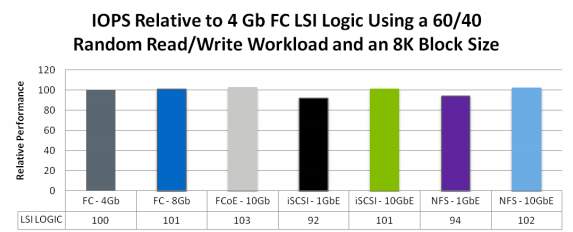
\includegraphics[width=\linewidth, keepaspectratio = true]{media/netapp_iops.png}
\mycaption{figure}{\label{abb:NetappIOPS}Netapp IOPS durchsatz für alle unterstützte Protokolle in Vergleich zu 4Gb FC mit 8K Block grösse\cite{Jafri2011}}
\end{center}

Der Report von Netapp hat ebenfalls die Latenz verglichen. Bei Latenz möchte man möglichst einen tiefen Wert erreichen. Gemäss \refabb{abb:NetappLatenz} ist die Latenz von iSCSI in einen 1 Gb Ethernet Netzwerk rund 9\% höher als bei Fibre Channel in einen 4Gb Netzwerk. Bei iSCSI in 10Gb Ethernet waren die Werte gleich wie Fibre Channel in 4Gb Netzwerk. Fibre Channel in einen 8Gb Netzwerk hatte jedoch rund 1\% tiefere Werte.\cite{Jafri2011}

\begin{center}
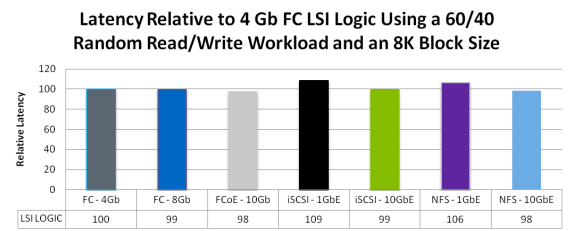
\includegraphics[width=\linewidth, keepaspectratio = true]{media/netapp_latence.png}
\mycaption{figure}{\label{abb:NetappLatenz}Netapp Latenz für alle unterstützte Protokolle in Vergleich zu 4Gb FC mit 8K Block grösse \cite{Jafri2011}}
\end{center}
 


\subsubsection{Skalierbarkeit Datenzugriffe}
Logical Units können im SAN zwar an Mehren Computersystemen zugeteilt werden, damit ist jedoch nicht sichergestellt, dass die Computersysteme gleichzeitig von gleichem Volume lesen geschweige drauf schreiben kann. Konventionelle Dateisysteme wie Ext3 gehen von einer exklusiven Nutzung des Speichers aus, weshalb diese keine Funktionen implementiert haben, die den gleichzeitigen Zugriff regeln. Schreiben zwei Computersysteme gleichzeitig in dieselbe Datei, kann nicht sichergestellt werden, welche Änderung gültig ist, was zu inkonsistent führt. Ein Dateisystem, welches den gleichzeitigen Zugriff erlaubt, muss Dateien, welche geändert werden, von der Änderung weiteren Computersystemen gesperrt (locking) werden. Cluster Dateisysteme wie Red Hat Global Filesystem (GFS) und Red Hat Global Filesystem 2 (GFS2) unterstützen dieses Sperren.



\subsubsection*{Skalierbarkeit Datenvolumen}
Durch den Einsatz eines Volume Manager können mehre Logical Unit zu einer grossen Logischen Volume zusammengefasst werden. Bei Linux Logical Volume Manager (LVM) können Logische Volumes bei einen 64Bit System von theoretisch 8 Exabyte erstellt werden. Das Dateisystem von Red Hat GFS bis Version 2 unterstützen theoretisch bei einen 64Bit System 8 Exabyte, Red Hat gibt jedoch einen Support von maximal 100 Terabyte.\cite{Levine2011}


\subsubsection{Standortübergreifend}
Für standortübergreifende Verfügbarkeit der Daten kann bei Block-Basierten Architekturen die serverseitige Spiegelung (Host-Based Mirroring) eingesetzt werden. Dazu sind pro Standort ein Speichersystem und der Einsatz eines Volume Manager. Bei Linux kann hier für Logical Volume Manager (LVM) eingesetzt werden. Bei LVM werden auf alle Logical Units mit einem Phyiscal-Volume-Label geschrieben, die daraus resultierenden Physical-Volumes werden zu einer Volume-Group zusammengefasst. Aus der Volume Group lässt sich ein oder mehre Logical Volume bilden, welche über die Standorte gespiegelt sind. Im Logical Volume 
wird schlussendlich ein Dateisystem installiert, welches normal im Linux eingehängt (mount) werden.

\subsubsection{Integrität}


\subsubsection{Backup}
Die Daten können mit Herkömmlichen Backup Verfahren gesichert werden.





